%%%%%%%%%%%%%%%%%%%%%%%%%%%%%%%%%%%%%
%                                   %
% Compile with XeLaTeX and biber    %
%                                   %
% Questions or comments:            %
%                                   %
% joshua dot mcneill at uga dot edu %
%                                   %
%%%%%%%%%%%%%%%%%%%%%%%%%%%%%%%%%%%%%

\documentclass{beamer}
  % Read in standard preamble (cosmetic stuff)
  %%%%%%%%%%%%%%%%%%%%%%%%%%%%%%%%%%%%%%%%%%%%%%%%%%%%%%%%%%%%%%%%
% This is a standard preamble used in for all slide documents. %
% It basically contains cosmetic settings.                     %
%                                                              %
% Joshua McNeill                                               %
% joshua dot mcneill at uga dot edu                            %
%%%%%%%%%%%%%%%%%%%%%%%%%%%%%%%%%%%%%%%%%%%%%%%%%%%%%%%%%%%%%%%%

% Beamer settings
% \usetheme{Berkeley}
\usetheme{CambridgeUS}
% \usecolortheme{dove}
% \usecolortheme{rose}
\usecolortheme{seagull}
\usefonttheme{professionalfonts}
\usefonttheme{serif}
\setbeamertemplate{bibliography item}{}

% Packages and settings
\usepackage{fontspec}
  \setmainfont{Charis SIL}
\usepackage{hyperref}
  \hypersetup{colorlinks=true,
              allcolors=blue}
\usepackage{graphicx}
  \graphicspath{{../../figures/}}
\usepackage[normalem]{ulem}
\usepackage{enumerate}

% Document information
\author{M. McNeill}
\title[FREN2001]{Français 2001}
\institute{\url{joshua.mcneill@uga.edu}}
\date{}

%% Custom commands
% Lexical items
\newcommand{\lexi}[1]{\textit{#1}}
% Gloss
\newcommand{\gloss}[1]{`#1'}
\newcommand{\tinygloss}[1]{{\tiny`#1'}}
% Orthographic representations
\newcommand{\orth}[1]{$\langle$#1$\rangle$}
% Utterances (pragmatics)
\newcommand{\uttr}[1]{`#1'}
% Sentences (pragmatics)
\newcommand{\sent}[1]{\textit{#1}}
% Base dir for definitions
\newcommand{\defs}{../definitions}


  % Packages and settings
  \usepackage[style=apa, backend=biber]{biblatex}
    \addbibresource{../references/References.bib}

  % Document information
  \subtitle[Dialectology]{Dialectology}

  %% Custom commands
  \newcommand{\regscale}{0.35}
  % Subsection/frame title
  \newcommand{\suboneone}{What are we talking about?}
  \newcommand{\subonetwo}{What's so important about geography?}
  \newcommand{\subonethree}{Origin of American dialects}
  \newcommand{\subonefour}{The North}
  \newcommand{\subonefive}{New England}
  \newcommand{\subonesix}{The South}
  \newcommand{\suboneseven}{Appalachia}
  \newcommand{\suboneeight}{The Midland}
  \newcommand{\subonenine}{The West}
  \newcommand{\suboneten}{Discussion}

\begin{document}
  % Read in the standard intro slides (title page and table of contents)
  %%%%%%%%%%%%%%%%%%%%%%%%%%%%%%%%%%%%%%%%%%%%%%%%%%%%%%%%%%%%%%%%
% This is a standard set of intro slides used in for all slide %
% documents. It basically contains the title page and table of %
% contents.                                                    %
%                                                              %
% Joshua McNeill                                               %
% joshua dot mcneill at uga dot edu                            %
%%%%%%%%%%%%%%%%%%%%%%%%%%%%%%%%%%%%%%%%%%%%%%%%%%%%%%%%%%%%%%%%

\begin{frame}
  \titlepage
  \tiny{Office: % Basically a variable for office hours location
Gilbert 121\\
        Office hours: % Basically a variable for office hours
 lundi, mercredi, vendredi 10:10--11:10
}
\end{frame}

\begin{frame}
  \tableofcontents[hideallsubsections]
\end{frame}

\AtBeginSection[]{
  \begin{frame}
    \tableofcontents[currentsection,
                     hideallsubsections]
  \end{frame}
}


  \section{Dialectology}
    \subsection{\suboneone}
      \begin{frame}{\suboneone}
        \begin{block}{Would you expect these two people to speak the same?}
          \begin{enumerate}
            \item A 20 year old, white, working-class female from \alert<2->{Georgia} in a casual conversation
            \item A 20 year old, white, working-class female from \alert<2->{Wisconsin} in a casual conversation
          \end{enumerate}
        \end{block}
        \begin{alertblock}<2->{Dialectology}
          % Dialectology
The study of geographic language variation

        \end{alertblock}
      \end{frame}

    \subsection{\subonetwo}
      \begin{frame}{\subonetwo}
        \begin{block}{Which person do you care most about?}
          \begin{enumerate}
            \item @angrypoliticsguy from Idaho on Twitter
            \item Kanye West
            \item Your friend that you hang out with every weekend
          \end{enumerate}
        \end{block}
        \begin{alertblock}<2->{}
          Face-to-face interaction is given precedence
        \end{alertblock}
      \end{frame}

      \begin{frame}[t]{\subonetwo}
        \begin{alertblock}{Isogloss}
          % Isogloss
A geographic boundary between where different variants of a particular linguistic variable are used

          \only<2>{
            \begin{itemize}
              \item Often but not always associated with physical boundaries
              \item Multiple isoglosses in the same location form \alert{bundles}
              \item Bundles define dialect boundaries
            \end{itemize}
          }
        \end{alertblock}
        \only<1>{
          \begin{alertblock}{Linguistic variable}
            % Linguistic variable
A linguistic unit that is realized in different ways depending on extra-linguistic factors

            \begin{itemize}
              \item Notated with parentheses: e.g., (r)
            \end{itemize}
          \end{alertblock}
        }
        \only<3->{
          \begin{center}
            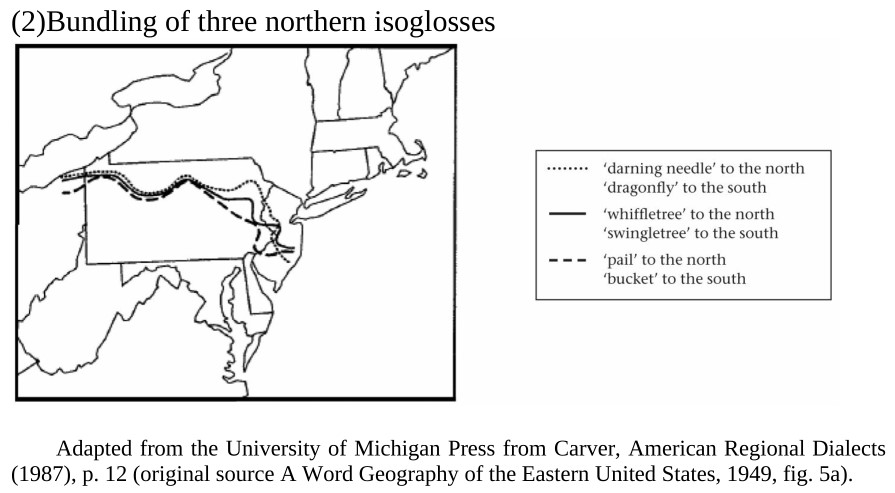
\includegraphics[scale=0.56]{pa_isogloss.jpg}
          \end{center}
        }
      \end{frame}

    \subsection{\subonethree}
      \begin{frame}{\subonethree}
        \begin{columns}
          \column{0.5\linewidth}
            \only<-2>{
              \begin{block}{Settlement patterns}
                \begin{itemize}
                  \item Colonists arrived from different parts of the UK
                  \item<2-> Colonists then spread out in different directions
                \end{itemize}
              \end{block}
            }
            \only<3>{
              \begin{block}{But it's not that simple}
                Colonists came into contact with:
                \begin{itemize}
                  \item Indian populations
                  \item Other European settlers
                  \begin{itemize}
                    \item French in LA, German in PA, Spanish in SW
                  \end{itemize}
                  \item African slaves who shaped the southern states
                \end{itemize}
              \end{block}
            }
            \only<4->{
              \begin{block}{And even less simple}
                African-Americans later migrated to the northern cities and further shaped the dialects there
              \end{block}
            }
          \column{0.5\linewidth}
            \only<1>{
              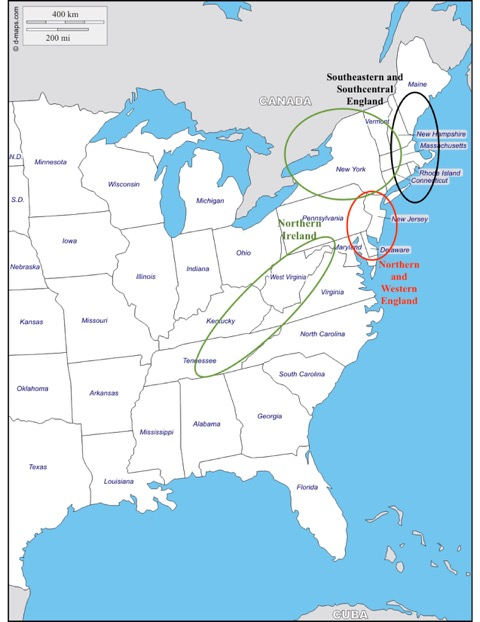
\includegraphics[scale=0.3]{eastern_usa1.jpg}
            }
            \only<2->{
              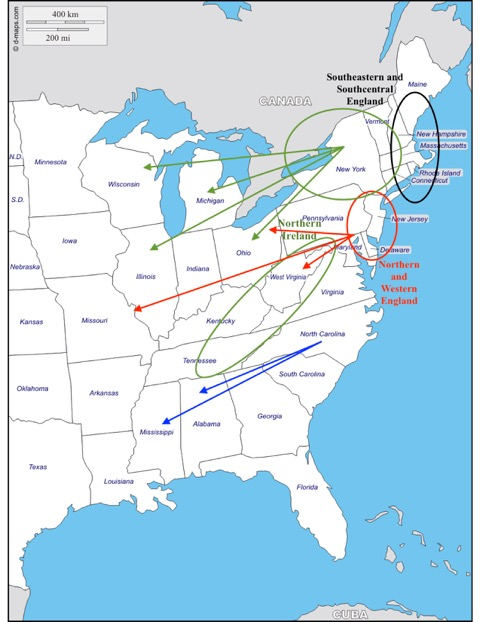
\includegraphics[scale=0.3]{eastern_usa2.jpg}
            }
        \end{columns}
      \end{frame}

      \begin{frame}[t]{\subonethree}
        \begin{center}
          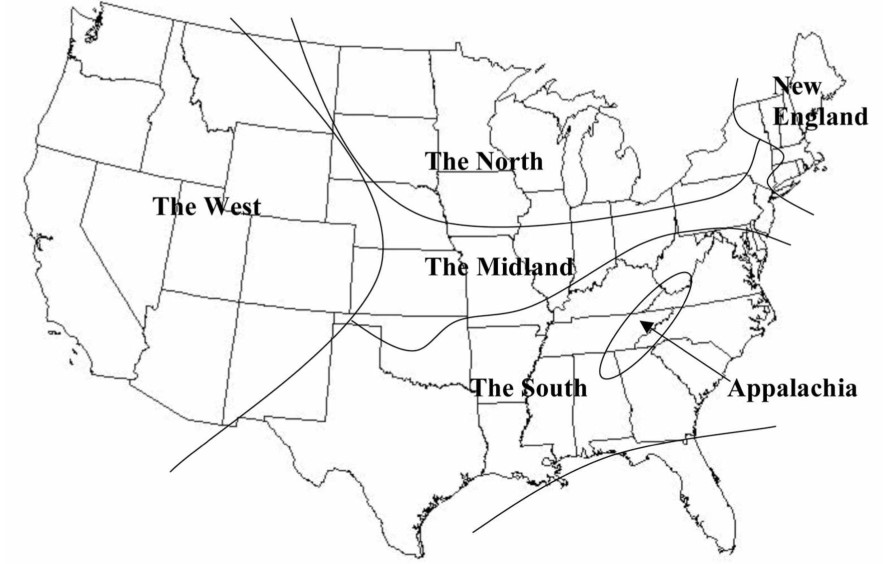
\includegraphics[scale=\regscale]{supraregional_dialects.jpg}
        \end{center}
        \only<1>{
          \begin{block}{The resulting dialect regions}
            \begin{itemize}
              \item Homogenized a bit for the middle-class
              \item Stable for the working-class \parencite{schneider_american_1997,labov_atlas_2006}
            \end{itemize}
          \end{block}
        }
        % \only<2->{
        %   \begin{block}{Doctrine of first effective settlement \parencite{zelinsky_cultural_1992}}
        %     The first group to settle an area has an outsized influence on the culture that develops there
        %   \end{block}
        % }
      \end{frame}

    \subsection{\subonefour}
      \begin{frame}{\subonefour}
        \begin{columns}
          \column{0.5\linewidth}
            \begin{minipage}[t][0.6\textheight]{\linewidth}
              \begin{block}{Some features}
                \only<1>{
                \begin{itemize}
                  \item \href{https://youtu.be/9UoJ1-ZGb1w?t=59}{The northern cities vowel shift}
                  \item \alert{Chain shift}: % Chain shift
A sound change that involves a domino effect where a change in one sounds causes a change in another and so on

                \end{itemize}
                }
                \only<2>{
                  Gerunds where \lexi{to be} constructions are expected
                  \begin{enumerate}
                    \item The table needs cleaning
                    \item The table needs to be cleaned
                  \end{enumerate}
                  \lexi{By} where \lexi{at} is expected
                  \begin{enumerate}
                    \setcounter{enumi}{2}
                    \item I was by Sarah's house
                    \item I was at Sarah's house
                  \end{enumerate}
                }
              \end{block}
            \end{minipage}
          \column{0.5\linewidth}
            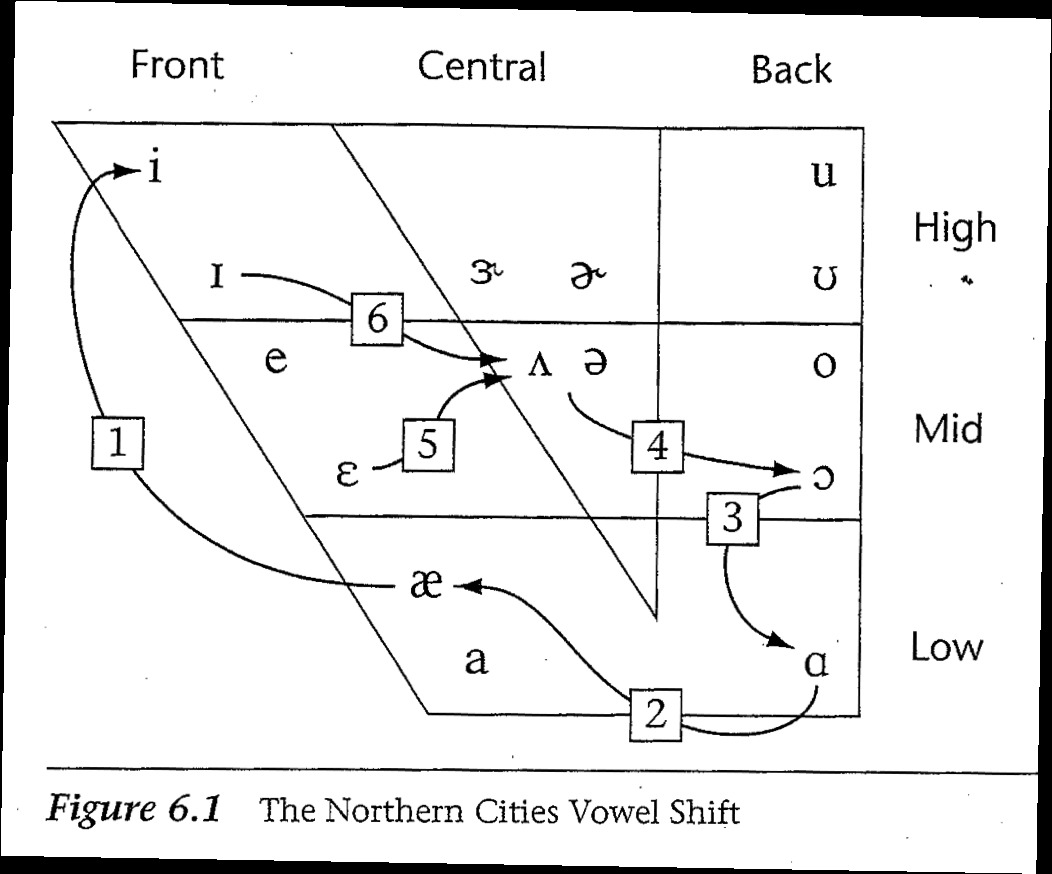
\includegraphics[scale=0.125]{northern_cities_shift.jpg}
        \end{columns}
      \end{frame}

      \begin{frame}{\subonefour}
        \begin{center}
          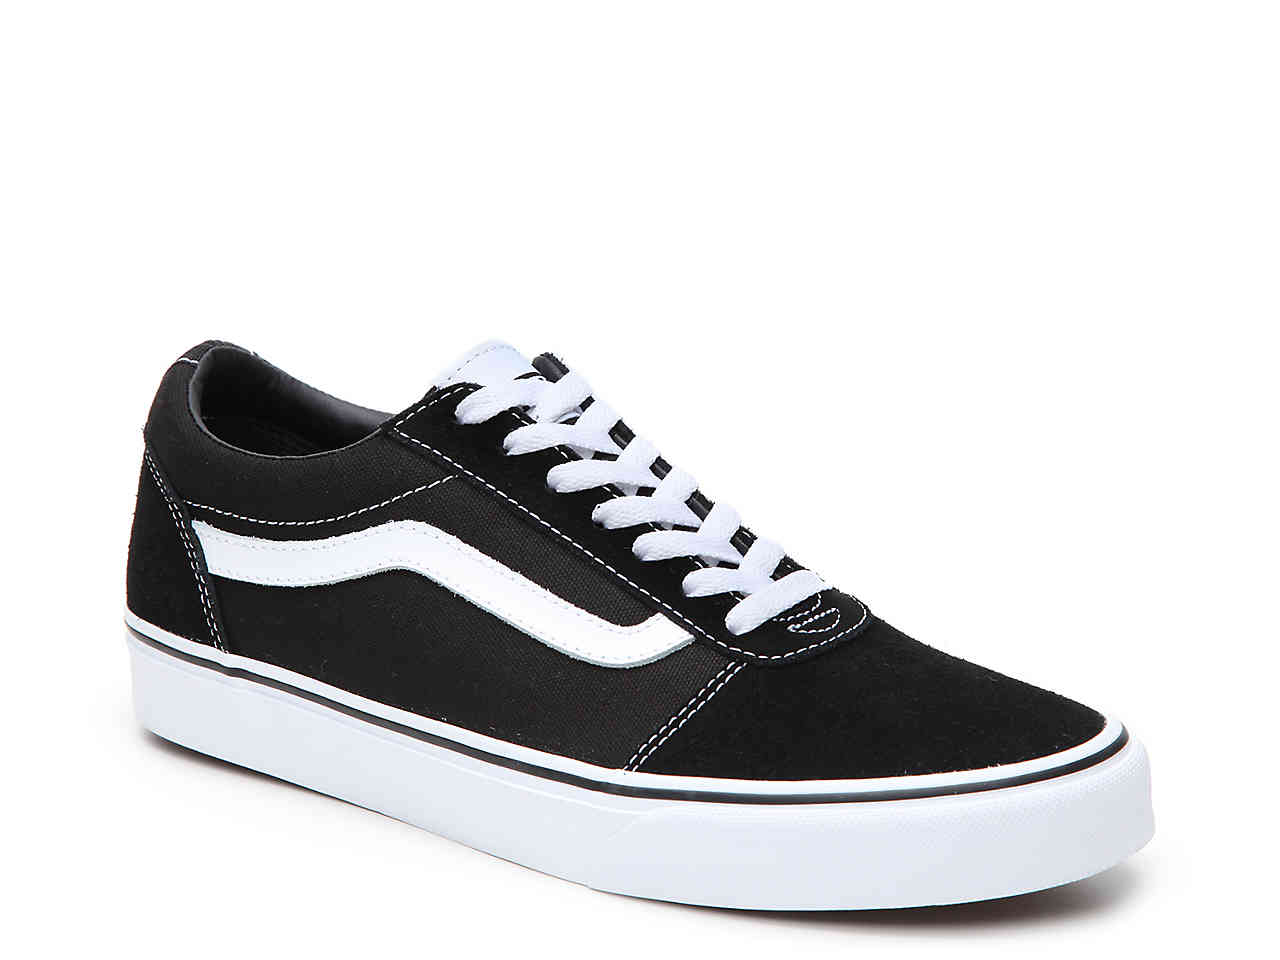
\includegraphics[scale=0.15]{sneaker.jpg}
        \end{center}
        \begin{block}{What do you call this?}
          \uncover<2->{
            sneaker
          }
        \end{block}
      \end{frame}

      \begin{frame}{\subonefour}
        \begin{columns}
          \column{0.5\linewidth}
            \begin{block}{What do you call this?}
              \uncover<2->{
                pop
              }
            \end{block}
          \column{0.5\linewidth}
            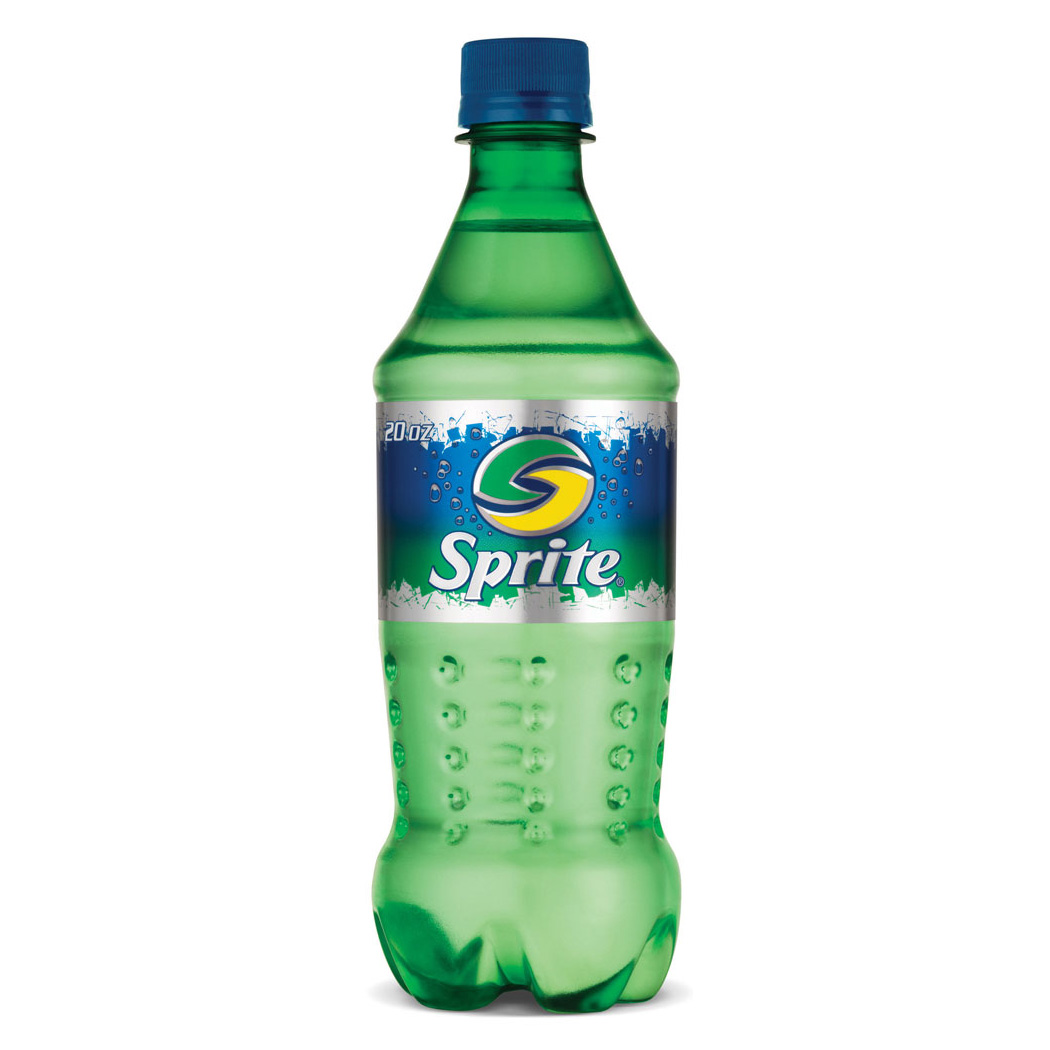
\includegraphics[scale=0.175]{sprite.jpg}
        \end{columns}
      \end{frame}

      \begin{frame}{\subonefour}
        \begin{center}
          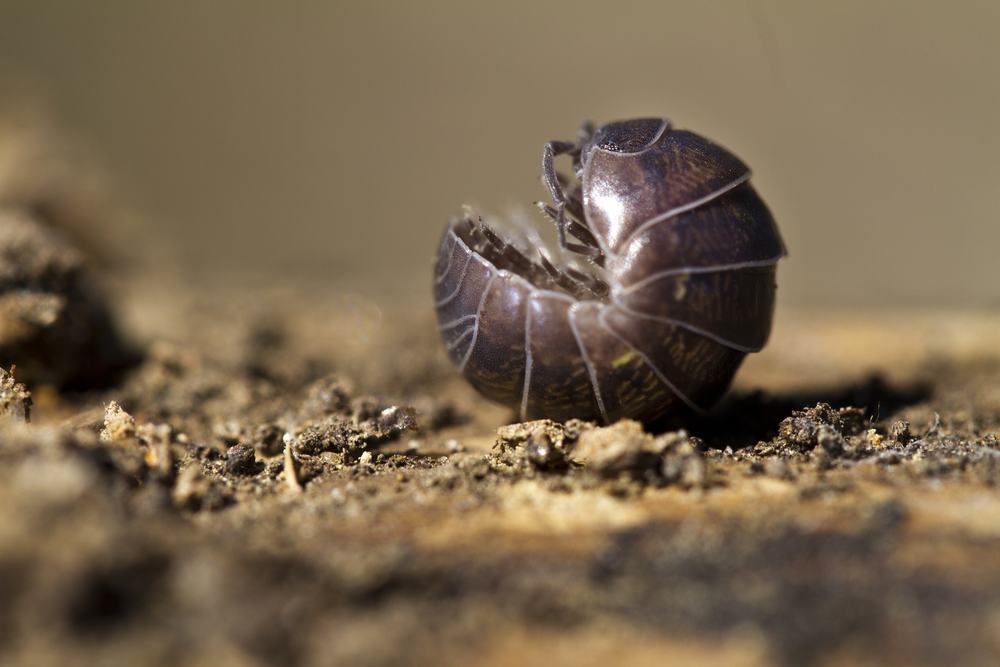
\includegraphics[scale=0.9]{roly-poly.jpg}
        \end{center}
        \begin{block}{What do you call this?}
          \uncover<2->{
            roly-poly
          }
        \end{block}
      \end{frame}

    \subsection{\subonefive}
      \begin{frame}[t]{\subonefive}
        \begin{center}
          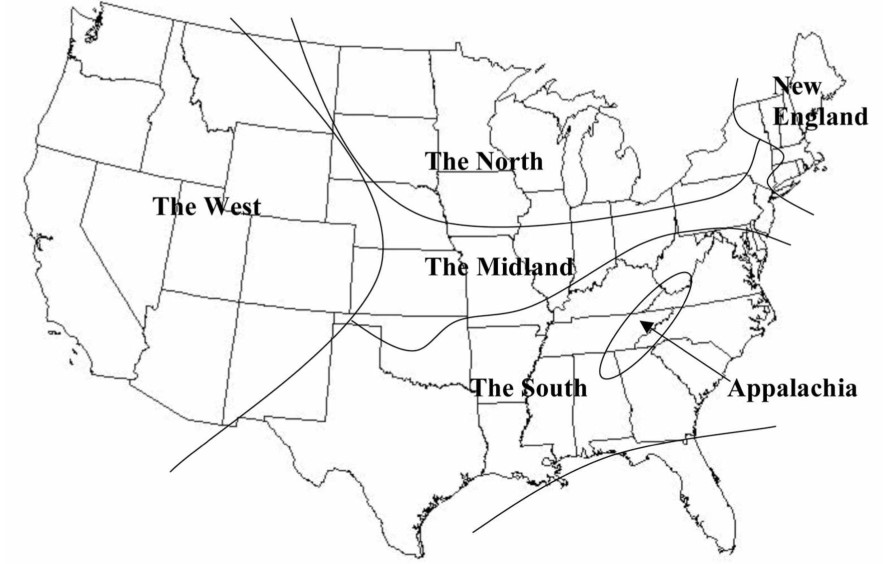
\includegraphics[scale=\regscale]{supraregional_dialects.jpg}
        \end{center}
        \only<1>{
          \begin{block}{The \textsc{cot-caught} merger}
            \lexi{Cot} and \lexi{caught} are both [ˈkɑt]
            \begin{itemize}
              \item \alert{Merger}: % Merger
A sound change that involves two phonemes coming to be only one phoneme

            \end{itemize}
          \end{block}
        }
        \only<2>{
          \begin{columns}
            \column{0.5\linewidth}
              \begin{block}{Non-rhotic}
                [ˈpʰɑːk jə ˈkʰɑː]
              \end{block}
            \column{0.5\linewidth}
              \begin{block}{To mark agreement}
                So don't I
              \end{block}
          \end{columns}
        }
        \only<3>{
          \begin{block}{Lexical differences}
            \parbox{0.48\linewidth}{
              \begin{enumerate}
                \item Waiting on line
                \item Waiting in line
              \end{enumerate}
            }
            \parbox{0.48\linewidth}{
              \begin{itemize}
                \item soda
                \item pill bug
              \end{itemize}
            }
          \end{block}
        }
      \end{frame}

      \begin{frame}{\subonefive}
        \begin{center}
          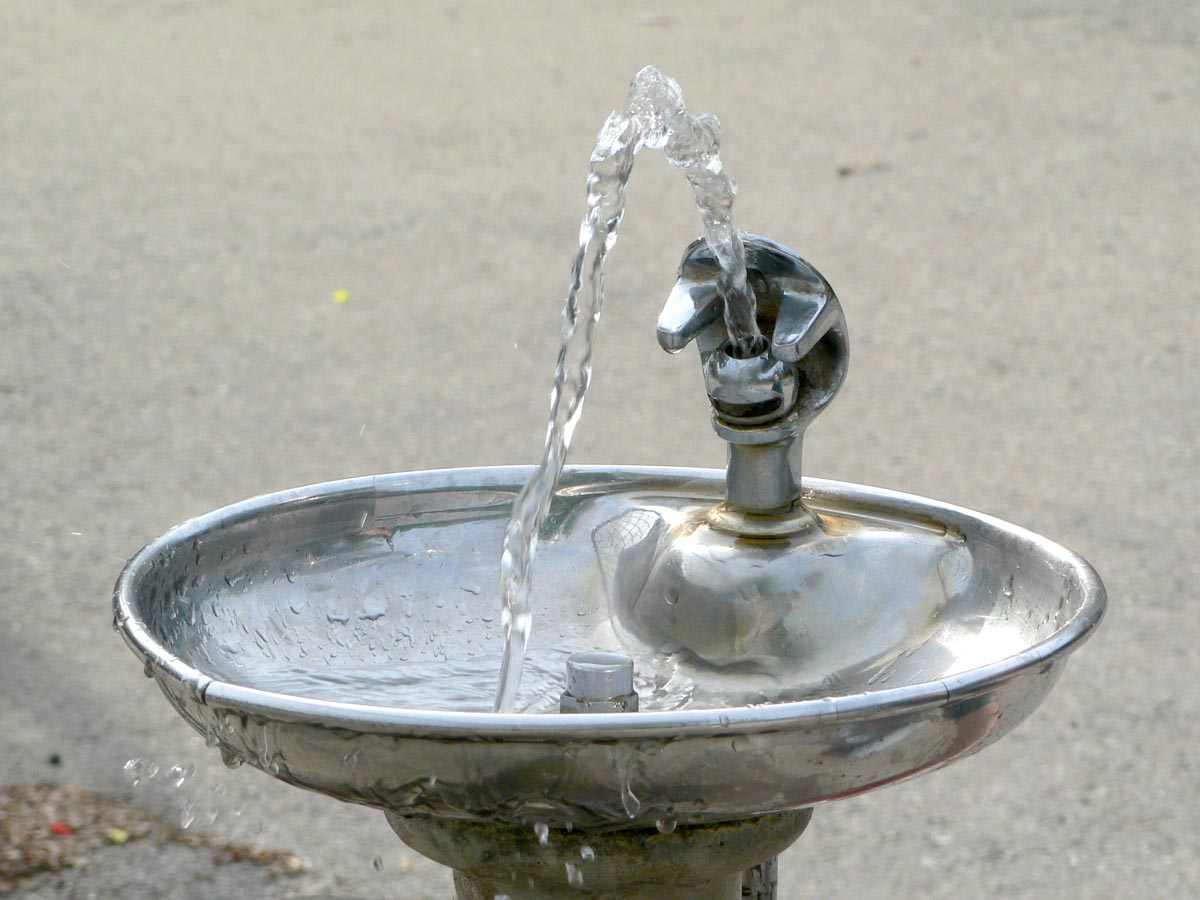
\includegraphics[scale=0.15]{bubbler.jpg}
        \end{center}
          \begin{block}{What would you call this?}
            \uncover<2->{
              bubbler
            }
          \end{block}
      \end{frame}

    \subsection{\subonesix}
      \begin{frame}[t]{\subonesix}
        \begin{center}
          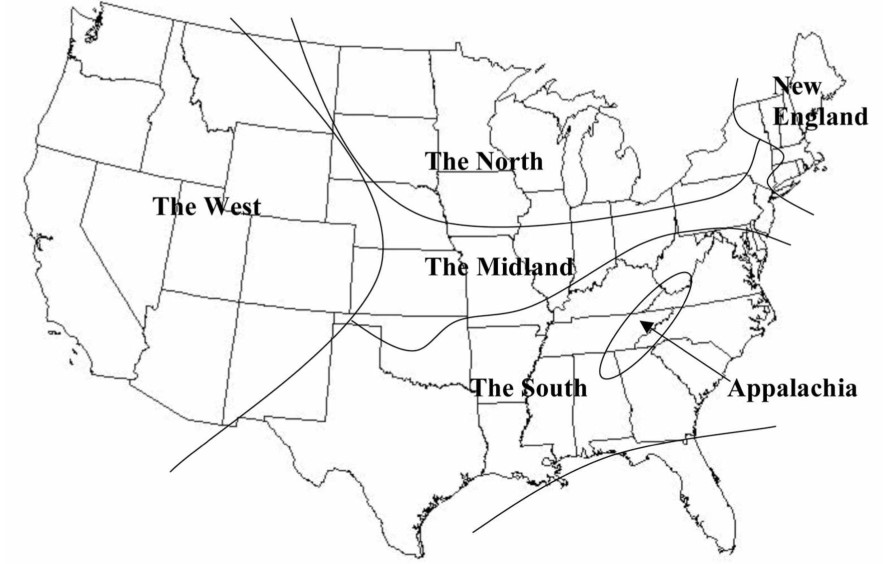
\includegraphics[scale=\regscale]{supraregional_dialects.jpg}
        \end{center}
        \only<-2>{
          \begin{block}{Diphthongization}
            How do you pronounce the vowel in \lexi{net}?
            \begin{itemize}
              \item<2-> {[}ˈnɛɪt]
              \item<2-> (ɪ) and (ɛ) are made into dipthongs
            \end{itemize}
          \end{block}
        }
        \only<3-4>{
          \begin{block}{Monophthongization}
            How do you pronounce the vowels in \lexi{wide} and \lexi{my}?
            \begin{itemize}
              \item<4-> {[}ˈwɑːd] and [ˈmɑː]
              \item<4-> The diphthong (aɪ) is often made into a monophthong
            \end{itemize}
          \end{block}
        }
        \only<5>{
          \begin{block}{The \textsc{pin-pen} merger \parencite{thomas_acoustic_2001}}
            \lexi{Pin} and \lexi{pen} are both [ˈpɪn]
            \begin{itemize}
              \item This is the case when the following consonant is /n/
            \end{itemize}
          \end{block}
        }
        \only<6>{
          \begin{block}{Morphosyntactic differences}
            \begin{enumerate}
              \item Fixin': I'm fixin' to clean the gutters
              \item Double modals: I might could clean the gutters
            \end{enumerate}
          \end{block}
        }
        \only<7>{
          \begin{block}{Lexical differences}
            \begin{itemize}
              \item coke
              \item roly-poly
            \end{itemize}
          \end{block}
        }
      \end{frame}

      \begin{frame}{\subonesix}
        \begin{columns}
          \column{0.5\linewidth}
            \begin{block}{What do you call this?}
              \uncover<2->{
                buggy
              }
            \end{block}
          \column{0.5\linewidth}
            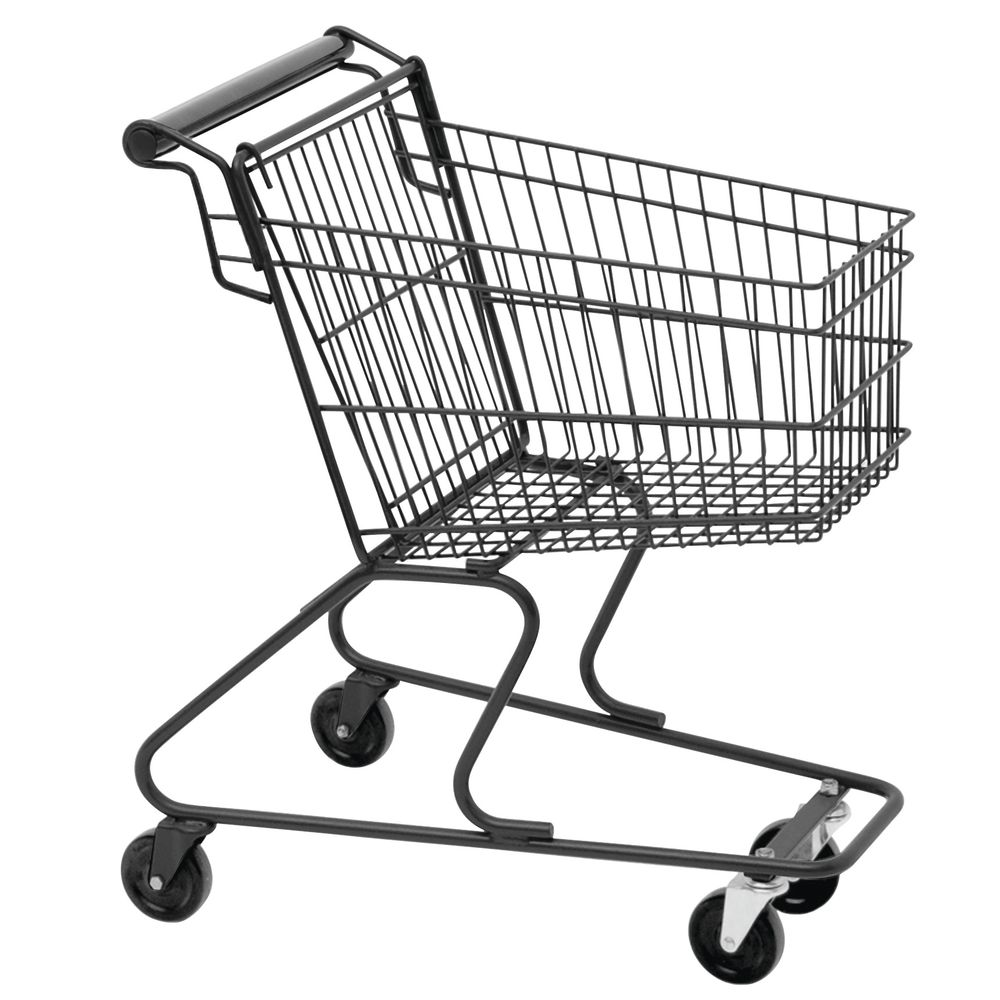
\includegraphics[scale=0.13]{buggy.jpg}
        \end{columns}
      \end{frame}

    \subsection{\suboneseven}
      \begin{frame}[t]{\suboneseven}
        \begin{center}
          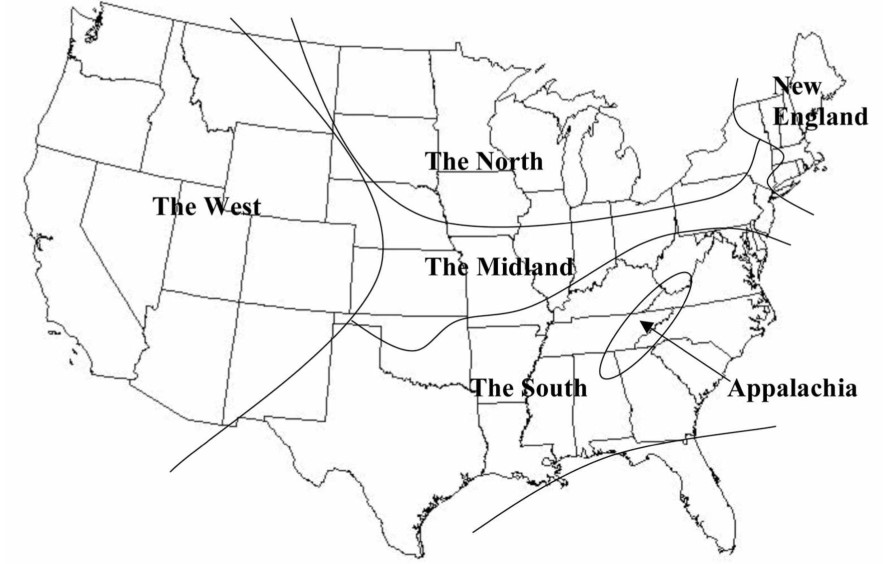
\includegraphics[scale=\regscale]{supraregional_dialects.jpg}
        \end{center}
        \only<1>{
          \begin{block}{(ɪ) and (ʊ) are tensed \parencite{brandes_dialect_1977}}
            \begin{itemize}
              \item \lexi{fish}: [ˈfiʃ]
              \item \lexi{push}: [ˈpuʃ]
            \end{itemize}
          \end{block}
        }
        \only<2>{
          \begin{block}{Primary stress on the first syllable \parencite{brandes_dialect_1977}}
            \begin{itemize}
              \item {[}ˈsɪ.ɡɑɹ] instead of [sɪˈɡɑɹ]
              \item {[}ˈnoʊ.vɛm.bɹ̩] instead of [noʊˈvɛm.bɹ̩]
            \end{itemize}
          \end{block}
        }
        \only<3>{
          \begin{block}{a-prefixing \parencite{wolfram_if_2006}}
            \begin{enumerate}
              \item He come a-running to tell me the news
              \item The dog was a-crying when he saw the deer
            \end{enumerate}
          \end{block}
        }
        \only<4>{
          \begin{block}{Apophony for past tense \parencite{wolfram_appalachian_1976}}
            \begin{itemize}
              \item {[}ˈklaɪm] $\rightarrow$ [ˈklʌm]
              \item {[}ˈhit] $\rightarrow$ [ˈhɛt]
              \item {[}ˈreɪk] $\rightarrow$ [ˈrʌk]
            \end{itemize}
          \end{block}
        }
        \only<5>{
          \begin{block}{Negative concord \parencite{brandes_dialect_1977}}
            I didn't have no lunch
            \begin{itemize}
              \item Questionably regional
            \end{itemize}
          \end{block}
        }
        \only<6>{
          \begin{block}{Lexical differences \parencite{montgomery_dictionary_2004}}
            \begin{itemize}
              \item \lexi{dope}: carbonated beverage
              \item \lexi{jasper}: an outsider
              \item \lexi{poke}: bag or sack
            \end{itemize}
          \end{block}
        }
      \end{frame}

    \subsection{\suboneeight}
      \begin{frame}[t]{\suboneeight}
        \begin{center}
          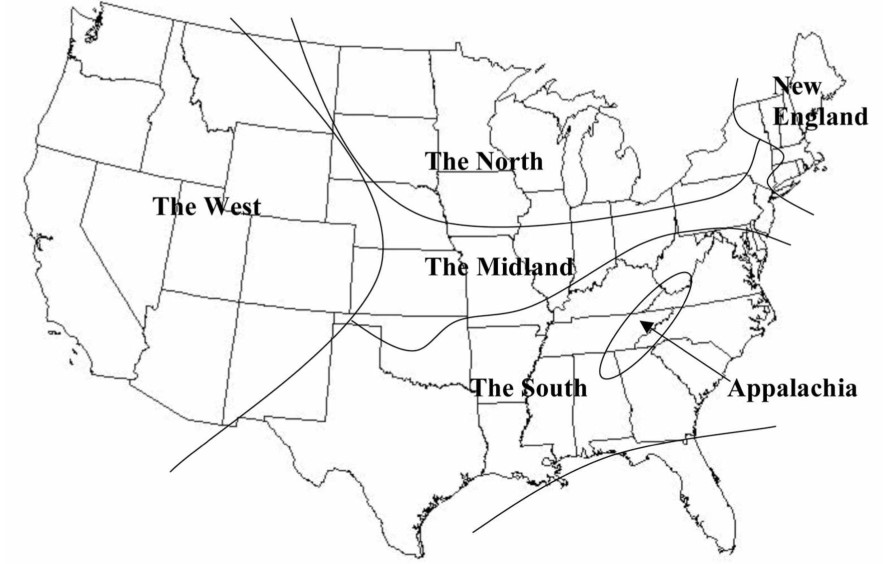
\includegraphics[scale=\regscale]{supraregional_dialects.jpg}
        \end{center}
        \only<1>{
          \begin{alertblock}{}
            This region doesn't exactly include NJ and eastern PA
          \end{alertblock}
        }
        \only<2>{
          \begin{block}{The dipthong (oʊ) as [øʊ] \parencite{thomas_acoustic_2001}}
            \parbox{\linewidth}{
              Which words are these?
            }
            \parbox{0.48\linewidth}{
              \begin{itemize}
                \item {[}ˈbøʊt]
              \end{itemize}
            }
            \parbox{0.48\linewidth}{
              \begin{itemize}
                \item {[}ˈmøʊ]
              \end{itemize}
            }
          \end{block}
        }
        \only<3>{
          \begin{block}{l-vocalization \parencite{dodsworth_attribute_2005}}
            \parbox{\linewidth}{
              Which words are these?
            }
            \parbox{0.48\linewidth}{
              \begin{itemize}
                \item {[}ˈhɪw]
              \end{itemize}
            }
            \parbox{0.48\linewidth}{
              \begin{itemize}
                \item {[}ˈbɛwt]
              \end{itemize}
            }
          \end{block}
        }
        \only<4>{
          \begin{block}{Near merger of \textsc{cot-caught} \parencite{durian_new_2012,labov_atlas_2006}}
            There is still some differentiation between (ɑ) and (ɔ)
          \end{block}
        }
        \only<5-6>{
          \begin{block}{Morphosyntactic differences}
            \only<5>{
              \begin{enumerate}
                \item Positive anymore: \uttr{It seems to rain every weekend anymore.} \parencite{frazer_positive_1993}
                \item All the further: \uttr{Johnstown was all the further I could drive.} \parencite{frazer_use_1993}
              \end{enumerate}
            }
            \only<6>{
              \begin{enumerate}
                \setcounter{enumi}{2}
                \item Verbed: \uttr{The table needs washed.} \parencite{murray_need_1996}
              \end{enumerate}
            }
          \end{block}
        }
        \only<7>{
          \begin{block}{Lexical differences}
            \begin{itemize}
              \item pop
              \item potato bug
            \end{itemize}
          \end{block}
        }
      \end{frame}

      \begin{frame}{\suboneeight}
        \begin{columns}
          \column{0.5\linewidth}
            \begin{block}{What do you call this?}
              \uncover<2->{
                sweeper
              }
            \end{block}
          \column{0.5\linewidth}
            
\includegraphics[scale=0.13]{sweeper.jpg}
        \end{columns}
      \end{frame}

    \subsection{\subonenine}
      \begin{frame}[t]{\subonenine}
        \begin{center}
          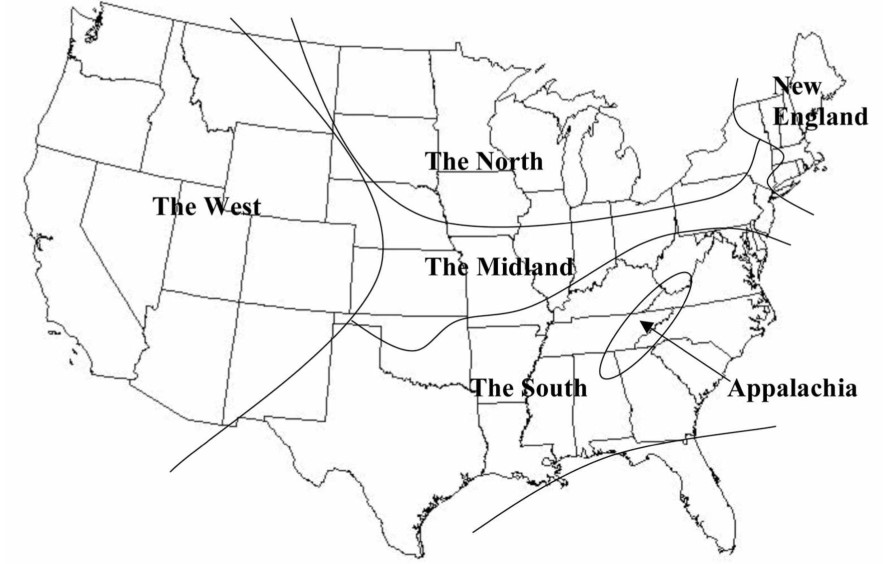
\includegraphics[scale=\regscale]{supraregional_dialects.jpg}
        \end{center}
        \only<-2>{
          \begin{block}{Phonological differences}
            \only<1>{
              \begin{itemize}
                \item \textsc{cot-caught} merger
                \item (u) is fronted so that \lexi{dude} is [ˈdʉd] \parencite{preston_national_2003}
              \end{itemize}
            }
            \only<2>{
              \begin{itemize}
                \item (ɪ) as [i]: \lexi{thing} [ˈθiŋ]
                \item (ɪ) as [ɛ]: \lexi{hid} [ˈhɛd] \parencite{eckert_vowel_nodate}
              \end{itemize}
            }
          \end{block}
        }
        \only<3>{
          \begin{block}{Quotative \lexi{like} and \lexi{all} \parencite{wolfram_getting_2006}}
            \begin{itemize}
              \item \uttr{I'm like, ``I don't have a crush on Kim.''}
              \item \uttr{I'm all, ``No he didn't.''}
            \end{itemize}
          \end{block}
        }
      \end{frame}

      \begin{frame}[t]{\subonenine}
        \begin{center}
          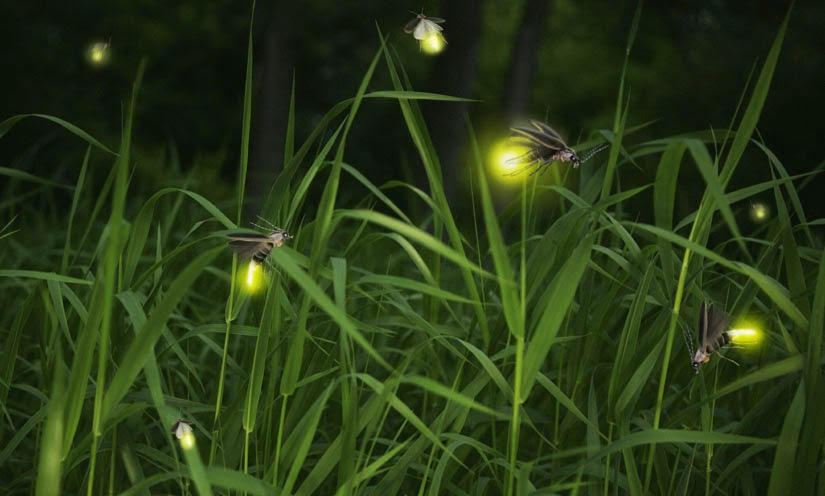
\includegraphics[scale=0.19]{firefly.jpg}
        \end{center}
        \only<-2>{
          \begin{block}{What would you call these?}
            \begin{itemize}
              \item<2-> \lexi{fireflies}
            \end{itemize}
          \end{block}
        }
        \only<3->{
          \begin{block}{Other lexical differences}
            \begin{itemize}
              \item \lexi{soda}
              \item \lexi{lookie lou}: traffic jam caused by people looking at an accident
              \item \lexi{granola}: a healthy person
            \end{itemize}
          \end{block}
        }
      \end{frame}

    \subsection{\suboneten}
      \begin{frame}{\suboneten}
        \begin{block}{}
          How accurate were these descriptions for you?
        \end{block}
      \end{frame}

      \begin{frame}[allowframebreaks]{References}
        \printbibliography
      \end{frame}
\end{document}
